%---------------------------------------------------------------------------------------------------
% Modellierung
%---------------------------------------------------------------------------------------------------
\section{Modellierung}\label{sec:modellierung}

Das Experiment besteht grob aus drei Phasen:
\begin{itemize}
  \item Aufstieg im Ballon
  \item Absprung und freier Fall
  \item Gebremster Fall am Fallschirm und Landung
\end{itemize}
Der Aufstieg wird im Rahmen dieser Arbeit nicht weiter betrachtet.
Interessanter ist der Fall - vor allem der ungebremste Abschnitt von Absprung bis zum Öffnen des Fallschirms.
Um dies zu simulieren, müssen relevante Kräfte und Größen berücksichtigt werden. %identifiziert und modelliert werden.

Seitenwinde und mögliche Rotation werden nicht modelliert.
Als Masse für Springer und Ausrüstung werden $140kg$ angeommen.
Auf den Springer und seine Ausrüstung wirken lediglich zwei Kräfte:
\begin{description}
  \item[$F_g$] Zur Erde hin wirkt die Gravitation.
  \item[$F_w$] Bremsend wirkt der Luftwiderstand.%, der sich bei Öffnen des Fallschirms massiv erhöht.
\end{description}

Die ausschlaggebenden Größen werden im Folgenden beschrieben.

\subsection{Gravitation}
Die Gravitation wirkt zwischen dem Springer und der Erde.
Allgemein wird hier das newtonsches Gravitationsgesetz angewendet.
\begin{equation}
F_g=G \frac{m_1 m_2}{r^2}
\end{equation}
Dabei ist $G$ die Gravitationskonstante $66.7384\times 10^{-12} \frac{m^3}{kg\ s^2}$, $m_1$ und $m_2$ die beteiligten Massen und $r$ deren Abstand.
Bis auf $r$ (der Springer bewegt sich ja auf die Erde zu) sind hier alle Größen konstant.
$r$ ist dabei gleich dem Radius der Erde $r_E$ plus der Höhe des Springers $h$ \vgl Abb.~\ref{fig:gravitation}.
\begin{figure}[h]
  \centering
  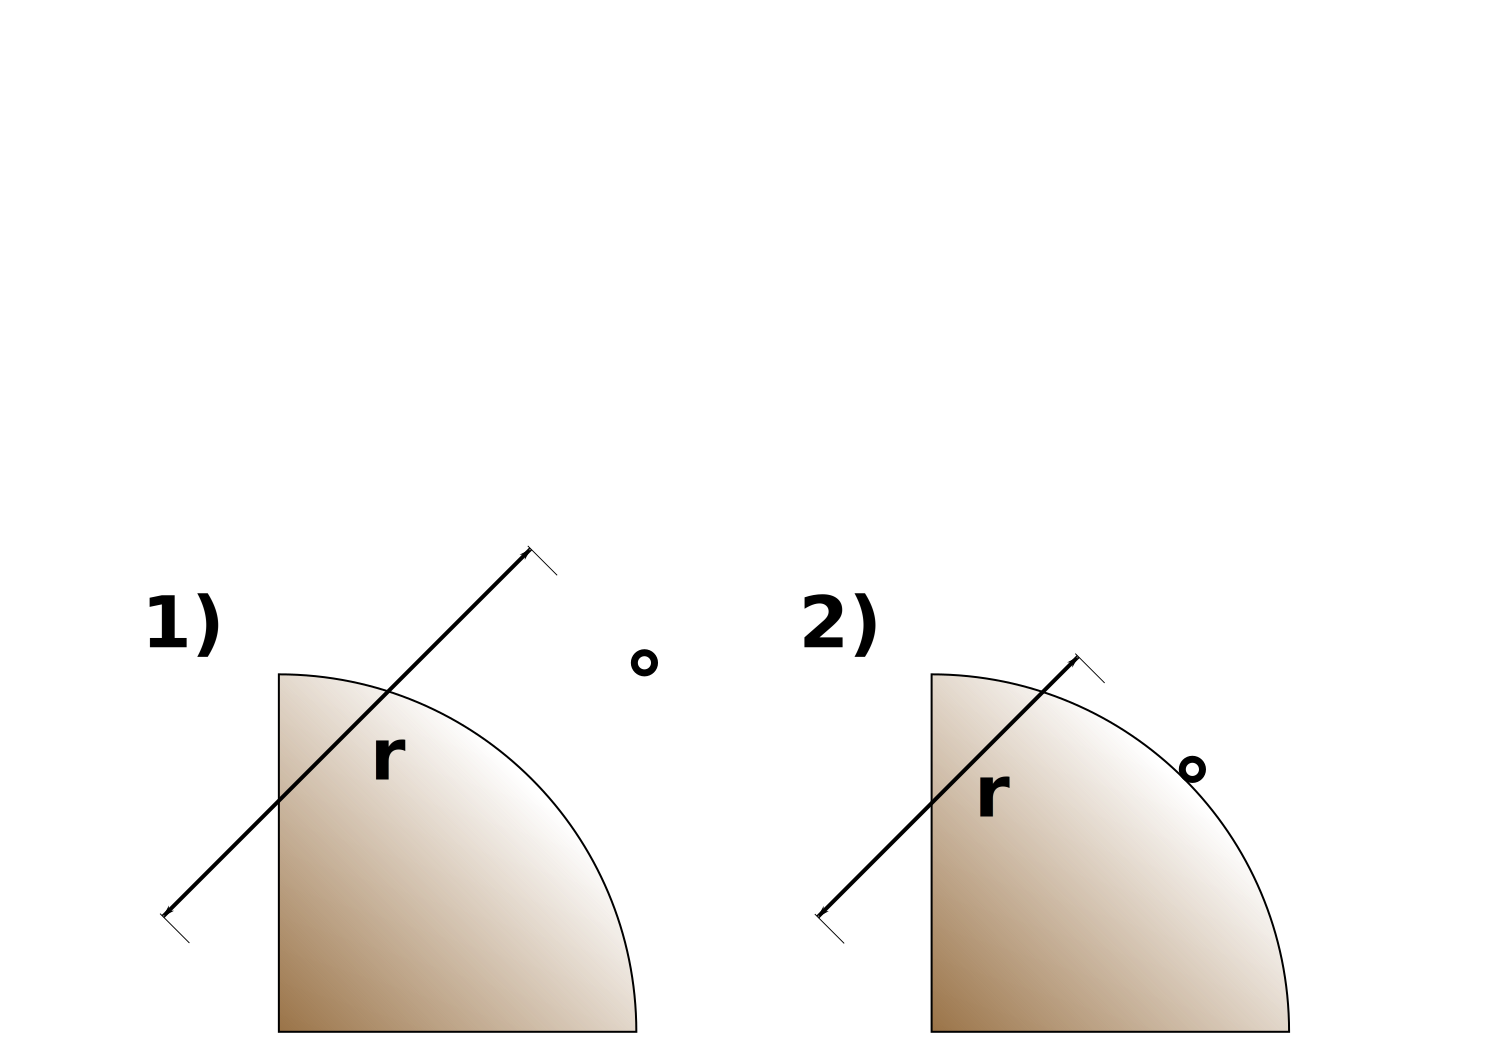
\includegraphics[width=0.5\textwidth]{gravitation}
  \caption{$r$ bei 1) Absprung und 2) Landung}
  \label{fig:gravitation}
\end{figure}

Als Erdradius wird der Äquatorradius $r_E=6 378 137m$ angenommen, als Masse des Springers $m_S=140kg$, als Masse der Erde $m_E=5.9736\times 10^{24}kg$.
Die Kraft, die auf den Springer auf Erdniveau herrscht beträgt
\begin{eqnarray}
F_{g_0} &=& 66.7384\cdot 10^{-12} \frac{140\cdot 5.9736\cdot 10^{24}}{6 378 137^2} \\
 &=& 1372 N \nonumber
\end{eqnarray}
Die Challenger zerbrach in $15km$ Höhe, der Sprung Baumgartners erfolgte aus knapp $40km$.
Um den Effekt der Höhenänderung deutlich zu zeigen wird als zweiter Wert die Gravitationskraft in $40km$ Höhe berechnet.
\begin{eqnarray}
F_{g_1} &=& 66.7384\cdot 10^{-12} \frac{140\cdot 5.9736\cdot 10^{24}}{\left(6 378 137 + 40 000\right)^2} \\
 &=& 1354.9 N \nonumber
\end{eqnarray}
Die Gravitationskraft nimmt in Absprunghöhe gegenüber der auf Erdniveau herrschenden um knapp $2\%$ ab.
Die Veränderung ist nicht groß, wird aber in der Simulation berücksichtigt.

\subsection{Luftwiderstand}
Der Fall des Springers wird durch den von der Atmosphäre verursachten Luftwiderstand gebremst.
Zur Berechnung dieser Kraft wird die Formel für den Strömungswiderstand verwendet.
\begin{equation}
F_w=\frac{1}{2}pv^2c_wA
\end{equation}
In die Berechnung der Kraft gehen die aktuelle Geschwindigkeit $v$, der Strömungswiderstandskoeffizient $c_w$, die angeströmte Fläche $A$ und die Dichte des umgebenden Mediums $p$ ein.
Die Geschwindigkeit ist das Integral der Beschleunigung, ergibt sich also zu jedem Zeitpunkt aus der Simulation.
Die Wahl von $p$, $c_w$ und $A$ werden im Folgenden beschrieben.
%Die Widerstandsfläche ändert sich bei Öffnung des Fallschirms.
%Weiterhin steigt die Widerstandsfläche in der Nähe der dichte- und temperaturabhängigen Schallgeschwindigkeit an.

\paragraph{Atmosphärenmodell}
Mit steigender Höhe nimmt der Luftdruck ab, da die darüberliegende Gassäule kürzer und somit leichter wird.
Auch die Temperatur ist höhenabhängig.
Zunächst ist die Temperatur der Erdoberfläche der ausschlaggebende Faktor.
Mit zunehmender Höhe nimmt dieser Einfluss ab und die Temperatur sinkt.
Ab einer bestimmten Höhe nimmt die Temperatur wieder zu, da ein immer geringerer Anteil der Einstrahlung von darüberliegenden Atmosphärenschichten blockiert wird.
Die Höhe, ab der die Temperatur wieder steigt ist von vielen Faktoren wie zum Beispiel der Tages- und Jahreszeit abhängig.
Nach einiger Beschäftigung mit Meteorologie, der Schichtung der Atmosphäre, Höhenformeln, virtueller Temperatur usw.~\cite{met:einfuehrung, met:umwelt}, wurde für die Simulation auf die eigene Umsetzung eines Atmosphärenmodells verzichtet.

Für die Simulation von Dichte und Temperatur wird das empirische NRLMSISE-00-Modell~\cite{nrlmsise00:goddardspaceflightcenter} verwendet, das in Matlab und Simulink als Funktion und Block zur Verfügung steht~\cite{matlab:mrlmsise-00}.
Es liefert abhängig von den Parametern Datum, Uhrzeit und geographische Position in einem Höhenbereich von $0$ bis $100km$ Werte für Dichte und Temperatur.
Für die Simulation wird lediglich die Höhe variiert und die anderen Parameter mit Ort und Zeit des Baumgartner-Experiments konstant vorbelegt.
Dichte und Temperatur stehen also jeweils als Funktion der Höhe zur Verfügung.

\paragraph{Strömungswiderstandskoeffizient und -fläche}
Der $c_w$-Wert eines Menschen liegt laut Zatsiorsky~\cite[88]{humankinetics} lageabhängig in einer Spanne von $0.35$ bis $1.36$.
Die höheren Werte gelten dabei für Lagen quer zum Luftstrom, das niedere Ende des Spektrums für Lagen längs zum Luftstrom.
Auch die angeströmte Fläche $A$ ist von der Richtung des Luftstroms abhängig.
Da Felix Baumgartner kurz nach dem Absprung in Rotation geriet und somit nicht kontinuierlich kopfüber längs zum Luftstrom fiel, werden für die Simulation die Werte $c_w=1.3$ und $A=0.8$ geschätzt, was in etwa dem in \cite{redbulletin:stratosspecialde} auf Seite 59 genannten Wert $c_w\cdot A=1.07$ entspricht.

\subsection{Gesamtmodell}

\begin{figure}[h]
  \centering
  \includegraphics[width=0.5\textwidth]{forces}
  \caption{Wirkende Kräfte}
  \label{fig:forces}
\end{figure}
Die resultierende Kraft $F_S$ (in Richtung Höhe) auf den Springer ist die Luftreibung minus der Gravitationskraft.
$F_S$ lässt sich zerlegen in das Produkt von Beschleunigung des Springers $a_S$ und Masse des Springers $m_S$.
Diese Formel nach $a_S$ umgestellt ist die für die Simulation benötigte Gesamtgleichung.
\begin{eqnarray}
  F_S &=& F_w-F_g \\
  a_Sm_S &=& F_w-F_g \nonumber \\
  a_S &=& \frac{F_w-F_g}{m_S} \label{f:a_s}\\
   &=& \frac{\frac{1}{2}pv^2c_wA-G\frac{m_Sm_E}{(r_E+h)^2}}{m_S} \nonumber
\end{eqnarray}
Nach dem Absprung erfährt der Springer also voraussichtlich zunächst eine negative Beschleunigung ($F_g\gg F_w$) bis die Geschwindigkeit weit genug gestiegen ist und er in dichtere Atmosphärenschichten gefallen ist und dort zunehmend abgebremst wird ($F_g<F_w$).


